
\documentclass{resume}
\usepackage{dashrule}
\usepackage{xcolor}
\usepackage{fontawesome5}
\usepackage[most]{tcolorbox}
\usepackage{tabularx}

% 状态徽标
\definecolor{pubgreen}{RGB}{22,155,98}
\definecolor{preblue}{RGB}{25,118,210}
\definecolor{revieworange}{RGB}{217,95,2}
\definecolor{authorblue}{RGB}{30,94,180}
\definecolor{cofirstteal}{RGB}{0,137,123}
\definecolor{corpurple}{RGB}{126,87,194}
\definecolor{authorgray}{RGB}{105,105,105}
\newcommand{\statusbadge}[2]{%
  \begingroup
  \setlength{\fboxsep}{1pt}%
  \colorbox{#1!10}{\textcolor{#1}{\footnotesize\textsf{#2}}}%
  \endgroup
}
\newcommand{\Published}{\statusbadge{pubgreen}{已发表}}
\newcommand{\Preprint}{\statusbadge{preblue}{预印本}}
\newcommand{\UnderReview}{\statusbadge{revieworange}{在投}}
\newcommand{\FirstAuthor}{\statusbadge{authorblue}{一作}}
\newcommand{\CoFirstAuthor}{\statusbadge{cofirstteal}{共同一作}}
\newcommand{\CorrespondingAuthor}{\statusbadge{corpurple}{通讯}}
\newcommand{\OtherAuthor}{\statusbadge{authorgray}{其他作者}}

\ResumeName{王冶-吉林大学人工智能学院博士生-26年12月毕业}

\begin{document}
\ResumeContacts{
    \faUser\ \href{https://wangyephd.github.io/}{ \textcolor{blue}{Homepage}} \quad %
    \faPhone\ 189-4754-6618 \quad%
    \faWeixin\ wangye889905 \quad%
    \faEnvelope\ yewang22@mails.jlu.edu.cn \quad%
    \ResumeUrl{https://space.bilibili.com/1127990326?spm_id_from=333.1007.0.0}{\faTv\ \textcolor{blue}{PaperABC}} \\
    \vspace{3pt}
    \emph{\textbf{The magic you are looking for is in the work you are avoiding.}}
}

\ResumeTitle

\noindent
\begin{tcolorbox}[colback=gray!5!white, colframe=gray!30!white, boxrule=0.3pt, sharp corners, before skip=4pt, after skip=6pt, title={\textbf{过往个人总结}}]
本人主要从事\textbf{图像风格迁移、图像生成与编辑、多模态定制化生成、统一理解与生成}等方向研究。迄今共发表论文\textbf{8篇}，其中以\textbf{第一作者}身份发表论文\textbf{6篇}，包括\textcolor{black}{\textbf{2篇CCF-A类}}（CVPR 2025、AAAI 2025）和\textcolor{black}{\textbf{1篇CCF-B类}}（Graphical Models）。此外，作为第一作者\textbf{2026年在投论文2篇}（ICML, ECCV 2026），并参与\textbf{4篇合作论文}在投（ECCV 2026）。代表性成果包括构建\textbf{OmniStyle大规模可泛化风格迁移}、\textbf{OmniStyle2去风格化驱动的高保真风格迁移}、提出\textbf{SigStyle定制化风格迁移框架}等。所提出的人物定制化生成工作\textbf{DP-Adapter}获\textcolor{black}{\textbf{CAD/Graphics 2025最佳论文提名奖}}。曾在\textbf{阿里、昆仑万维、百度、京东}从事算法实习。 \\
现在\textbf{腾讯优图青云计划实习}。
\end{tcolorbox}


\section{\textbf{教育背景}}
\noindent
\begin{tabularx}{\linewidth}{@{}X r@{}}
  \textbf{吉林大学}，人工智能学院 \quad\textit{博士研究生在读}
    & \textcolor{gray}{2022 -- 至今} \\[0.2em]
  \textbf{吉林大学}，计算机科学与技术学院 \quad\textit{硕士}
    & \textcolor{gray}{2019 -- 2022} \\[0.2em]
  \textbf{大连海事大学}，信息科学技术学院 \quad\textit{本科}
    & \textcolor{gray}{2015 -- 2019} \\
\end{tabularx}

\vspace{5pt}


\section{\textbf{学术成果}}

% 说明：按成果状态归类，并保留作者身份信息。
\subsection*{{\textbf{已发表}}}
\begin{enumerate}
  \item \textbf{OmniStyle: Filtering High Quality Style Transfer Data at Scale}\\
  \FirstAuthor \quad \href{https://arxiv.org/pdf/2505.14028}{\textcolor{blue}{\textbf{Paper}}} \quad \textbf{CVPR 2025 (CCF-A)}

  \item \textbf{SigStyle: Signature Style Transfer via Personalized Text-to-Image Models}\\
  \FirstAuthor \quad \href{https://arxiv.org/pdf/2502.13997}{\textcolor{blue}{\textbf{Paper}}} \quad \textbf{AAAI 2025 (CCF-A)}

  \item \textbf{DP-Adapter: Dual-Pathway Adapter for Boosting Fidelity and Text Consistency in Customizable Human Image Generation}\\
  \FirstAuthor \quad \href{https://arxiv.org/abs/2502.13999}{\textcolor{blue}{\textbf{Paper}}} \quad \textbf{Graphical Models (CCF-B)}

  \item \textbf{SingleDream: Attribute-Driven T2I Customization from a Single Reference Image}\\
  \FirstAuthor \quad \href{https://dl.acm.org/doi/10.1007/978-981-96-5812-1_12}{\textcolor{blue}{\textbf{Paper}}} \quad \textbf{CVM 2025 (CCF-C)}

  \item \textbf{PairHuman: A High-Fidelity Photographic Dataset for Customized Dual-Person Generation}\\
  \CoFirstAuthor \quad \href{https://arxiv.org/pdf/2511.16712}{\textcolor{blue} {\textbf{Paper}}} \quad
  \textbf{Information Fusion（中科院一区）}

  \item \textbf{FreeControl: Efficient, Training-Free Structural Control via One-Step Attention Extraction}\\
  \OtherAuthor \quad \textbf{NeurIPS 2025 (CCF-A)}

  \item \textbf{3D-SSGAN: Lifting 2D Semantics for 3D-Aware Compositional Portrait Synthesis}\\
  \OtherAuthor \quad \textbf{Pacific Graphics 2024 (CCF-B)}

  \item \textbf{P2M2-Net: Part-Aware Prompt-Guided Multimodal Point Cloud Completion}\\
  \OtherAuthor \quad \textbf{CAD/Graphics 2023 (CCF-C)}
\end{enumerate}

\vspace{-5pt}

\subsection*{{\textbf{投稿中}}}
\begin{enumerate}
  \item \textbf{OmniStyle2: Learning to Stylize by Learning to Destylize}\\
  \FirstAuthor \quad \href{https://arxiv.org/pdf/2509.05970}{\textcolor{blue}{\textbf{Paper}}} \quad \textbf{ECCV 2026 在投}

  \item \textbf{Atelier: Agentic Artist-Grounded Image Generation from Underspecified Artistic Intent}\\
  \CoFirstAuthor \quad \textbf{ACL ARR 2026 在投}

  \item \textbf{MXM-CLR: A Unified Framework for Contrastive Learning of Multifold Cross-Modal Representations}\\
  \FirstAuthor \quad \href{https://arxiv.org/abs/2303.10839}{\textcolor{blue}{\textbf{Paper}}} \quad \textbf{IJCV 在投 (CCF-A)}

  \item \textbf{HPrefStyle: Human-Aligned Style Transfer via Preference Learning}\\
  \CorrespondingAuthor \quad \textbf{TMM 在投 （中科院一区）}

  \item \textbf{StyleMV: Unified Stylized Multi-View Image Generation}\\
  \OtherAuthor \quad \textbf{ECCV 2026 已投稿}
\end{enumerate}

\vspace{2pt}

\section{\textbf{主要合作者}}

\begin{center}
  \href{https://yilinwang.org/}{\textcolor{blue}{\textbf{Yilin Wang}}} \textcolor{gray}{(Adobe)} \quad $\cdot$ \quad
  \href{https://scholar.google.com/citations?user=EcS0L5sAAAAJ&hl=en}{\textcolor{blue}{\textbf{Mingdeng Cao}}} \textcolor{gray}{(Adobe)} \quad $\cdot$ \quad
  \href{https://scholar.google.com/citations?user=XC6Z56AAAAAJ&hl=en}{\textcolor{blue}{\textbf{Zili Yi}}} \textcolor{gray}{(Nanjing University)}
\end{center}
\vspace{-5pt}
\noindent\rule{\linewidth}{0.4pt}

\vspace{10pt}



\section{\textbf{当前科研项目}}

\vspace{8pt}

\begin{center}
\begin{minipage}[t]{0.245\linewidth}
\centering
\parbox[c][2.6em][c]{\linewidth}{\centering\textbf{统一模型的后训练}}\\
\vspace{3pt}
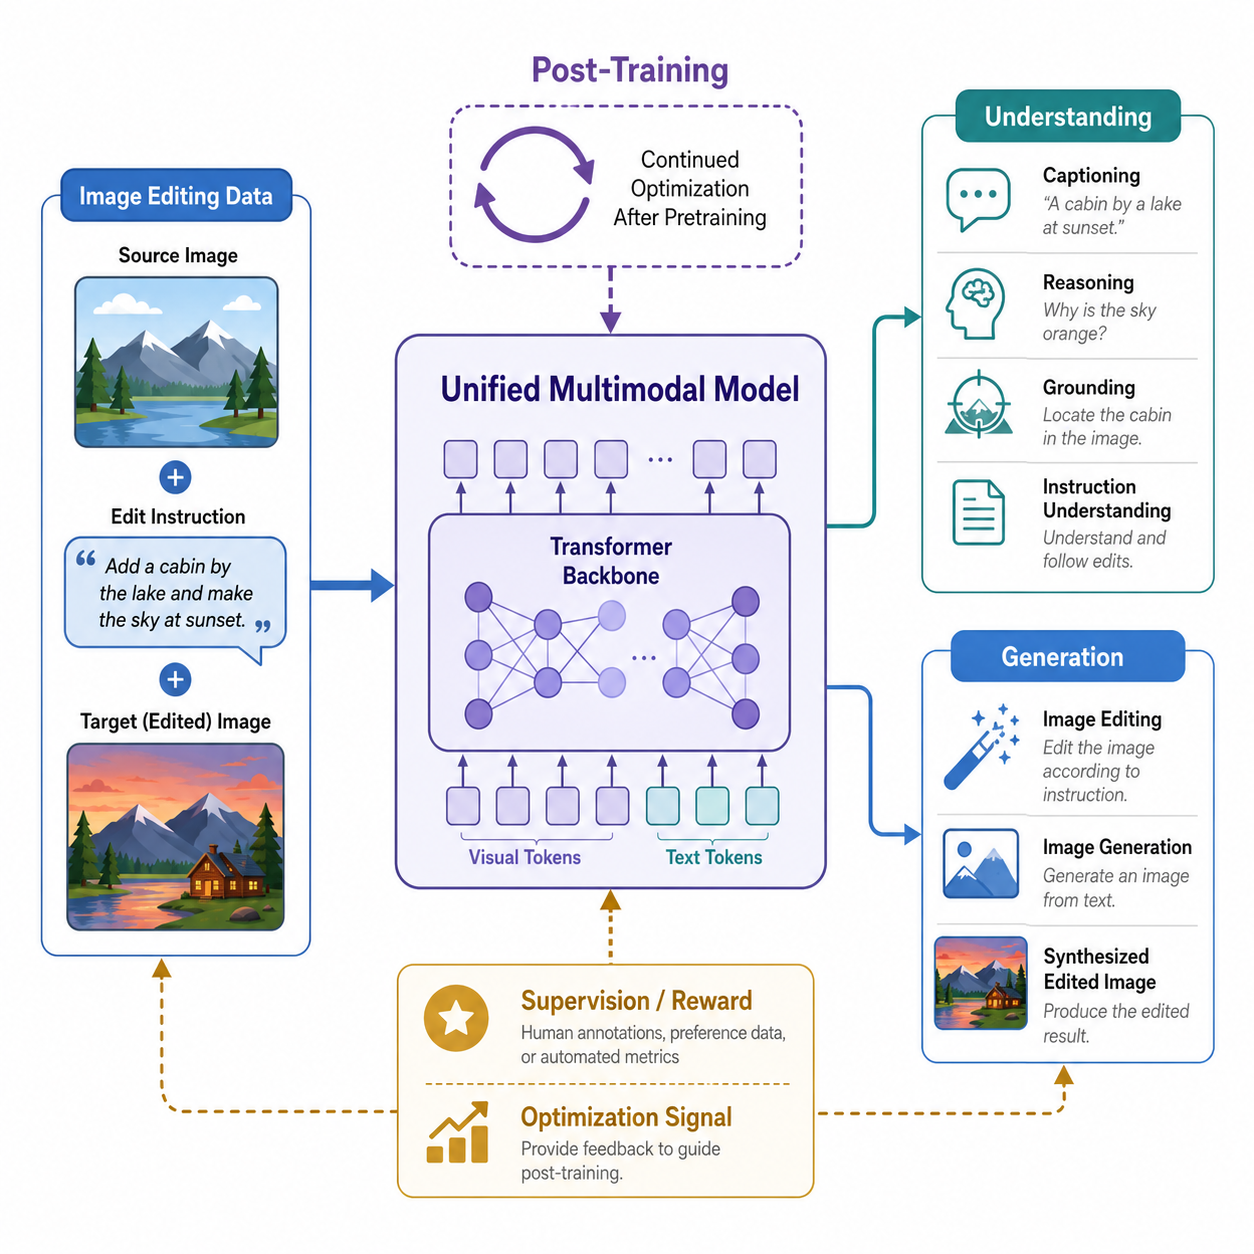
\includegraphics[width=0.96\linewidth,keepaspectratio]{figs/image.png}\\
\vspace{3pt}
\small 论文准备release中
\end{minipage}\hfill
\begin{minipage}[t]{0.245\linewidth}
\centering
\parbox[c][2.6em][c]{\linewidth}{\centering\textbf{OmniFont: 字体图像生成}}\\
\vspace{3pt}
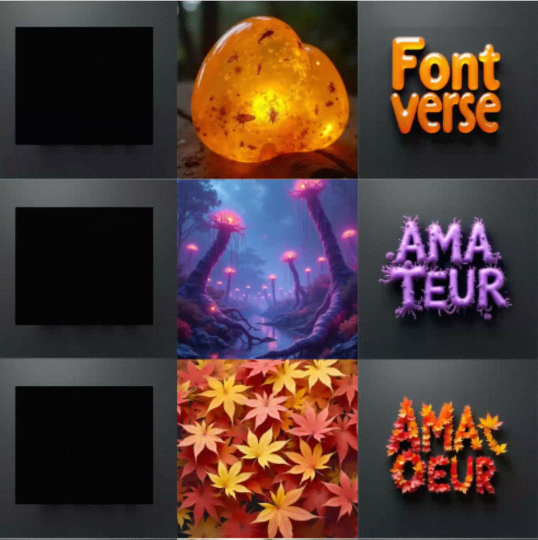
\includegraphics[width=0.96\linewidth,keepaspectratio]{figs/222.png}\\
\vspace{3pt}
\small 进行中
\end{minipage}\hfill
\begin{minipage}[t]{0.245\linewidth}
\centering
\parbox[c][2.6em][c]{\linewidth}{\centering\textbf{艺术图像智能体}}\\
\vspace{3pt}
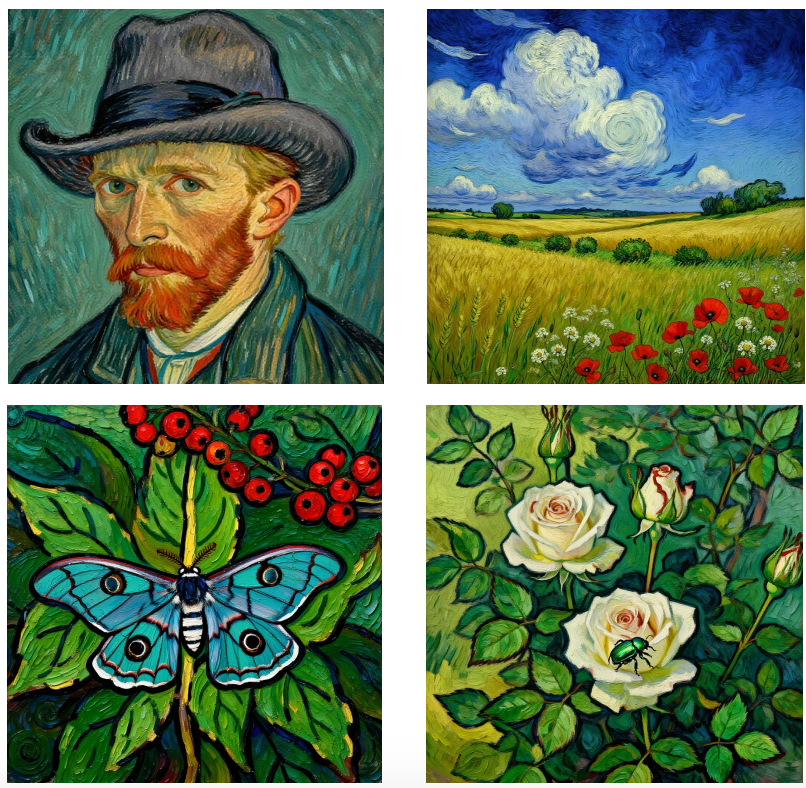
\includegraphics[width=0.96\linewidth,keepaspectratio]{figs/art1.png}\\
\vspace{3pt}
\small ACL ARR 2026投稿中
\end{minipage}\hfill
\begin{minipage}[t]{0.245\linewidth}
\centering
\parbox[c][2.6em][c]{\linewidth}{\centering\textbf{SVG图像生成}}\\
\vspace{3pt}
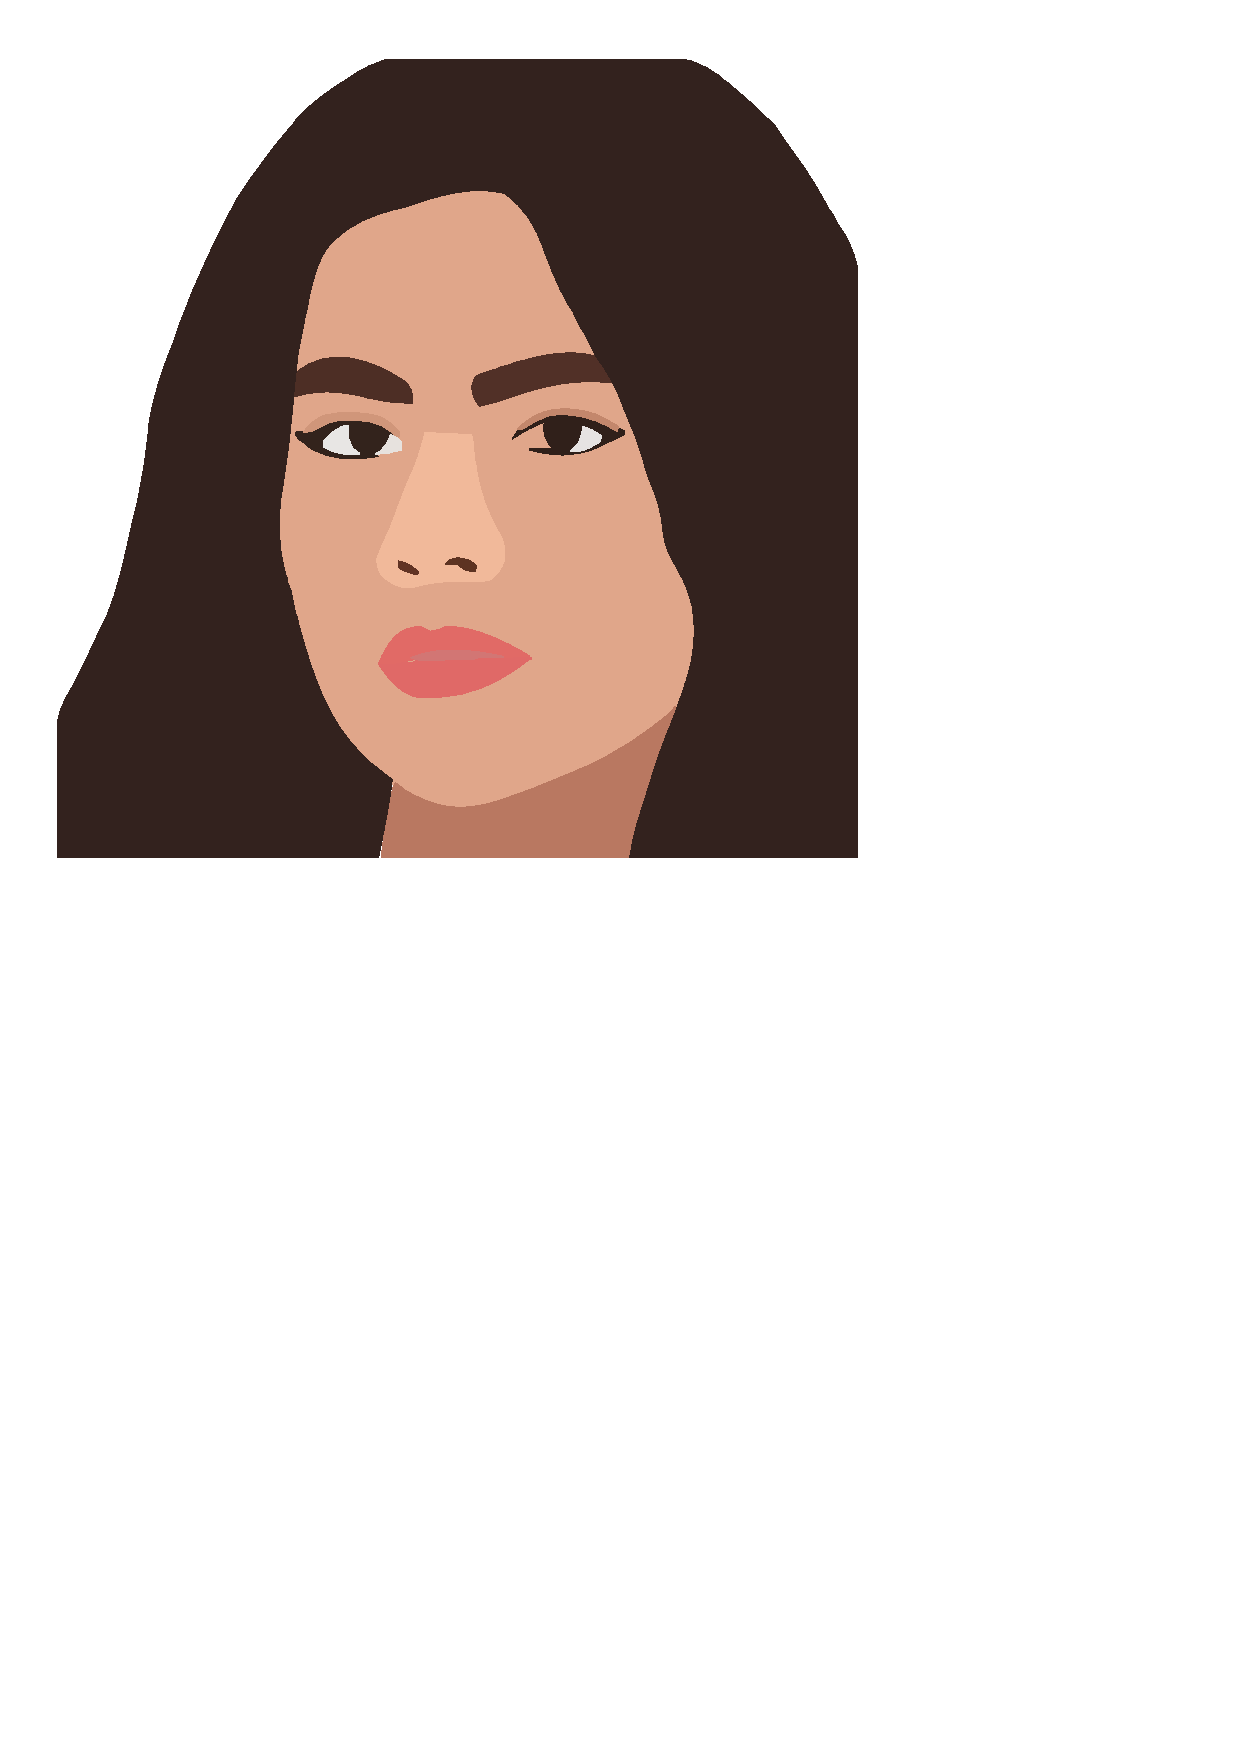
\includegraphics[width=0.96\linewidth,keepaspectratio]{figs/01340.jpg.pdf}\\
\vspace{3pt}
\small 进行中
\end{minipage}
\end{center}


\vspace{8pt}


\section{\textbf{实习经历}}


\noindent\textbf{腾讯优图}
\hfill \textcolor{gray}{2026.3—至今}

\noindent\textcolor{black}{神农研究中心} | \textbf{青云计划实习}

\begin{itemize}
  \item \textbf{项目内容：} Post-training for Unified Understanding and Generation Model
  \item \textbf{Mentor：} \href{https://scholar.google.com/citations?user=3to3lqMAAAAJ&hl=en}{\textcolor{blue}{\textbf{刘伟}}}
\end{itemize}

\vspace{0.4em}


\noindent\textbf{阿里巴巴}
\hfill \textcolor{gray}{2025.10—2026.1}

\noindent\textcolor{black}{AMAP Group} | 研究型算法实习生

\begin{itemize}
  \item \textbf{项目内容：} Physical-Aware Image Generation
  \item \textbf{Mentor：} \href{https://scholar.google.com/citations?user=rAtlzLcAAAAJ&hl=zh-CN}{\textcolor{blue}{\textbf{王永}}}
\end{itemize}

\vspace{0.4em}

\noindent\textbf{昆仑万维}
\hfill \textcolor{gray}{2024.03—2024.06}

\noindent\textcolor{black}{AI Story部门} | 研究型算法实习生

\begin{itemize}
  \item \textbf{项目内容：}多主体人物图像生成算法研发
  \item \textbf{技术栈：}深度学习、图像生成
  \item \textbf{Mentor：} \href{https://scholar.google.com/citations?user=XC6Z56AAAAAJ&hl=en}{\textcolor{blue}{\textbf{易子立}}}
\end{itemize}

\vspace{0.4em}

\noindent\textbf{百度}
\hfill \textcolor{gray}{2021.03—2021.06}

\noindent\textcolor{black}{百度地图} | 数据挖掘算法实习生

\begin{itemize}
  \item \textbf{项目内容：}实时公交ETA预估优化、公交发车间隔预估
  \item \textbf{技术栈：}机器学习、时间序列分析、大数据处理
  \item \textbf{Mentor：} 荣岳成，徐之冕
\end{itemize}

\vspace{0.4em}

\noindent\textbf{京东}
\hfill \textcolor{gray}{2020.11—2021.01}

\noindent\textcolor{black}{京东数科} | 数据挖掘算法实习生

\begin{itemize}
  \item \textbf{项目内容：}灰色用户信息挖掘和识别系统开发
  \item \textbf{技术栈：}数据挖掘、用户画像、风险识别
\end{itemize}

\vspace{5pt}


\section{\textbf{其他亮点}}

\begin{itemize}
  \item \textbf{\textcolor{black}{学术自媒体运营：}} 
  
  \quad 运营 \ResumeUrl{https://space.bilibili.com/1127990326?spm_id_from=333.1007.0.0}{\textcolor{blue}{\textbf{PaperABC}}} 学术频道
  
  \begin{itemize}
    \item 运营时间：2023.01 至今
    \item 粉丝数量：\textbf{1.3万+} | 视频播放量：\textbf{28万+}
    \item 专注：AIGC前沿论文解读与技术分享
  \end{itemize}
\end{itemize}

\end{document}
